\documentclass{standalone}
\usepackage{mathpazo}

\usepackage{tikz}
\usetikzlibrary{calc}

\begin{document}

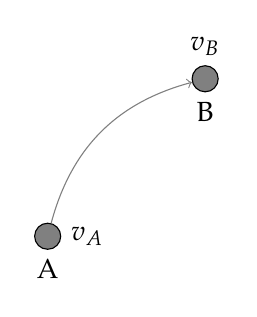
\begin{tikzpicture}
  \node[circle, draw=black,fill=gray,minimum size = 1pt,label=below:A, label=right:$v_A$] (A) at (0,0) {};
  \node[circle, draw=black,fill=gray,minimum size = 1pt,label=below:B, label=above:$v_B$] (B) at (2,2) {};
    \draw[->, gray] (A) edge[bend left] (B);
\end{tikzpicture}

\end{document}